\documentclass[border=10pt]{standalone}
\usepackage{tikz}
\usetikzlibrary{arrows.meta,positioning,calc,fit,backgrounds}
\usepackage{times}

\begin{document}
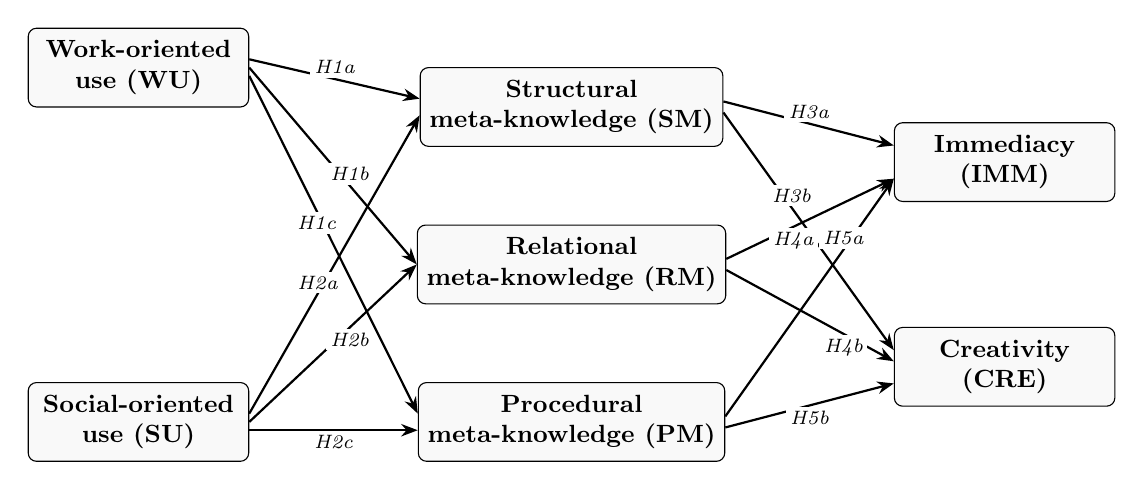
\begin{tikzpicture}[
  % Node styles
  iv/.style={draw, rounded corners=3pt, minimum width=2.8cm, minimum height=1cm,
             font=\small\bfseries, fill=gray!5, align=center},
  mk/.style={draw, rounded corners=3pt, minimum width=2.8cm, minimum height=1cm,
             font=\small\bfseries, fill=gray!5, align=center},
  dv/.style={draw, rounded corners=3pt, minimum width=2.8cm, minimum height=1cm,
             font=\small\bfseries, fill=gray!5, align=center},
  % Arrow style (all hypothesized paths use the same style)
  hyp/.style={-{Stealth[length=6pt]}, thick, black},
  % Label style
  lbl/.style={font=\scriptsize\itshape, fill=white, inner sep=1.5pt},
]

% === Column 1: IVs ===
\node[iv] (WU) at (0, 0) {Work-oriented\\use (WU)};
\node[iv] (SU) at (0, -4.5) {Social-oriented\\use (SU)};

% === Column 2: Mediators ===
\node[mk] (SM) at (5.5, -0.5) {Structural\\meta-knowledge (SM)};
\node[mk] (RM) at (5.5, -2.5) {Relational\\meta-knowledge (RM)};
\node[mk] (PM) at (5.5, -4.5) {Procedural\\meta-knowledge (PM)};

% === Column 3: DVs ===
\node[dv] (IMM) at (11, -1.2) {Immediacy\\(IMM)};
\node[dv] (CRE) at (11, -3.8) {Creativity\\(CRE)};

% === Stage 1 arrows: IV -> MK (6 arrows) ===
% WU paths
\draw[hyp] ([yshift=3pt]WU.east)  -- node[lbl, above]            {H1a} ([yshift=3pt]SM.west);
\draw[hyp] (WU.east)              -- node[lbl, above, pos=0.6]    {H1b} (RM.west);
\draw[hyp] ([yshift=-3pt]WU.east) -- node[lbl, below, pos=0.4]   {H1c} ([yshift=3pt]PM.west);

% SU paths
\draw[hyp] ([yshift=3pt]SU.east)  -- node[lbl, above, pos=0.4]   {H2a} ([yshift=-3pt]SM.west);
\draw[hyp] (SU.east)              -- node[lbl, below, pos=0.6]    {H2b} (RM.west);
\draw[hyp] ([yshift=-3pt]SU.east) -- node[lbl, below]             {H2c} ([yshift=-3pt]PM.west);

% === Stage 2 arrows: MK -> DV (6 arrows) ===
% SM paths
\draw[hyp] ([yshift=2pt]SM.east)  -- node[lbl, above]             {H3a} ([yshift=6pt]IMM.west);
\draw[hyp] ([yshift=-2pt]SM.east) -- node[lbl, above, pos=0.4]    {H3b} ([yshift=6pt]CRE.west);

% RM paths
\draw[hyp] ([yshift=2pt]RM.east)  -- node[lbl, below, pos=0.4]    {H4a} ([yshift=-6pt]IMM.west);
\draw[hyp] ([yshift=-2pt]RM.east) -- node[lbl, below, pos=0.7]    {H4b} ([yshift=2pt]CRE.west);

% PM paths
\draw[hyp] ([yshift=2pt]PM.east)  -- node[lbl, above, pos=0.7]    {H5a} ([yshift=-6pt]IMM.west);
\draw[hyp] ([yshift=-2pt]PM.east) -- node[lbl, below]              {H5b} ([yshift=-6pt]CRE.west);


\end{tikzpicture}
\end{document}
